\chapter{Cahier des charges}
\section{Remise en contexte}
\myparagraph{Les vulnérabilités de type Use-After-Free}
\subparagraph{}
La plupart des vulnérabilités enseignées et étudiées dans le cadre scolaire sont connues depuis longtemps.
On prendra comme exemple les dépassements de tampons, les problèmes de
formatage des chaines de caractères, etc.\subparagraph{}
Dans l'environnement industriel, et sur les solutions importantes utilisées dans le monde
de l'entreprise, ces vulnérabilités sont de plus en plus rares. Premièrement parce que le temps
faisant son œuvre, la grande majorité ont été reportées sur les solutions les plus anciennes,
mais également parce que de nombreux outils pouvant les détecter rapidement (parfois dès la compilation)
ont été conçus.\subparagraph{}
Les attaquants explorent donc de nouvelles voies, notamment sur des problématiques plus dynamiques, et/ou
liées également à l'environnement de production du programme, comme le système d'exploitation ou les bibliothèque utilisées.
En effet, de nombreuses opérations du programme dépendent intrinsèquement du système d'exploitation sous-jacent et
même si le comportement final reste souvent le même sur les différentes plateformes, les effets collatéraux
sur le contexte et le mécanisme d'exécution est souvent différent.\subparagraph{}
Une vulnérabilité de type usage-après-libération (\textbf{use-after-free}) consiste
en l'utilisation d'une zone mémoire après que celle ci ai été libérée.

\subparagraph{L'évolution des vulnérabilités de type use-after-free}
\begin{figure}[h]
    \centering
    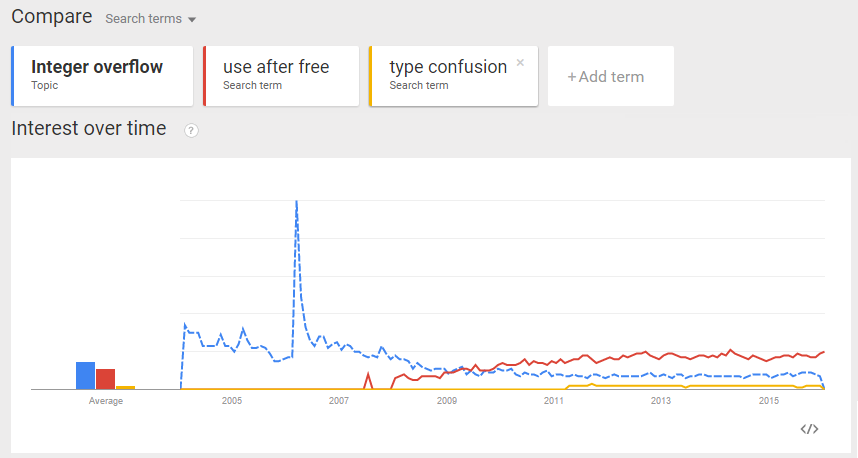
\includegraphics[scale=0.5]{images/histogramme-uaf.png}
    \caption{Evolution des vulnérabilités de type use-after-free.}
\end{figure}
Beaucoup de problèmes de corruption mémoire sont directement dûs à la mauvaise utilisation
du langage utilisé pour le développement. En effet, les langages de programmation tels que C
ou C++ demandent une gestion de la mémoire manuelle (le C++ permet néanmoins une gestion plus ou moins automatisée
avec les nouveaux standards).
\subparagraph{}
Il est donc fréquent de rencontrer des erreurs sur ce point là. Cela arrive
notamment lorsque par un problème de maintenabilité ou de mauvaise conception, la partie du programme devant
libérer une zone mémoire est méconnue/non documentée.\subparagraph{}
Ce n'est cependant pas toujours le cas et les allocateurs de mémoires / ramasse-miettes sont parfois en cause.

\subparagraph{Exemple}
Un exemple très simple et souvent rencontré dans la littérature est le suivant:
\begin{figure}[h]
    \centering
    \begin {lstlisting}[frame=single]
int main(void)
{
    int *a = malloc(sizeof(int));
    *a = 5;
    free(a);
    int *b = malloc(sizeof(int));
    printf("\%d", *b); // affiche 5
    *b = 7;
    printf("\%d", *b); // affiche 7
    *a = 10;
    printf("\%d", *b); // affiche 10
}
    \end{lstlisting}
    \caption{Exemple de use-after-free.}
\end{figure}
\subparagraph{}
Sur une distribution Linux classique comme Ubuntu, quelle que soit la taille de mots
de l'architecture (32 ou 64 bits), les adresses a et b sont exactement les mêmes.
Cela est directement dû à l'algorithme d'allocation mémoire de la bibliothèque standard
C.\subparagraph{}
En effet lors du premier appel à la fonction \textbf{malloc()}, une première zone est allouée.
Lors de sa libération, la zone libérée est mise en cache, et lors du second appel à \textbf{malloc()},
l'algorithme va retourner la même zone mémoire. Ce comportement ne sera pas détaillé dans cette section, car
il demanderait à lui seul plusieurs pages.\subparagraph{}
Cela va de soi que cet exemple est simpliste, et que les vulnérabilités rencontrées en production sont
rarement aussi visibles. Il permet toutefois de bien visualiser l'origine du problème.


\myparagraph{Outils existants en dynamique et en statique}
Des outils simplistes ne suffisent pas à détecter la présence d'use-after-free.\newline
Par exemple, si une solution détecte uniquement l'accès à une zone mémoire non allouée, l'exemple
donnée précédemment ne sera pas considéré comme vulnérable, car la zone mémoire est là même pour deux
allocations différentes. Plusieurs possibilités s'ouvrent alors : l'analyse statique, l'analyse dynamique,
et un mélange des deux.\subparagraph{}
On parle d'analyse dynamique lorsque l'analyse se déroule lorsque le programme s'exécute, et à l'inverse d'analyse statique lorsque celui-ci ne l'est pas.

\myparagraph{Analyse dynamique}
De nombreuses personnes / équipes se sont penchées sur la détection de ces comportements, dynamiquement et
statiquement. Nous parlerons tout d'abord des solutions dynamiques existantes, puis nous aborderons \textbf{les approches
statiques, qui sont directement liées au sujet de ce stage.}

\subparagraph{Kasan: Kernel Address Sanitizer}
Kasan\footnote{https://github.com/google/kasan} est un projet open-source, développé majoritairement
par les acteurs du noyaux Linux ainsi que par Google. Son but est d'ajouter une couche de protection
mémoire au noyau Linux afin de détecter certaines corruptions mémoires dans les opérations du noyau, comme
des use-after-free ou des accès hors limites.
https://github.com/google/kasan

\subparagraph{AddressSanitizer}
AddressSanitizer est également un projet open-source, et effectue
un travail similaire à Kernel Address Sanitizer mais côte utilisateur. Intégré dans la base de code de
LLVM, il permet, lorsque le programme testé est compilé avec les bonnes options du compilateur \textbf{Clang},
de détecter des problèmes de mémoires.

\subparagraph{Undangle}
Undangle est également un exemple connu, spécialement dédié à la découverte de vulnérabilité
de type use-after-free et double-free, à partir d'une trace d'exécution. Il a été développé par plusieurs
personnes travaillant à l'IMDEA Software Institute.

\myparagraph{Analyse statique}

De nombreux outils dynamiques détectant les problèmes liés à la mémoire existent et remplissent parfaitement leur rôle.
L'analyse dynamique a néanmoins plusieurs défauts.\newline

\subparagraph{Les avantages d'une analyse statique}

Lors de la phase de test d'une application, ainsi que lors de la recherche de vulnérabilités dans celle-ci, une bonne méthodologie
est d'essayer de parcourir tous les chemins possibles lors de l'exécution. Cela nécessite donc plusieurs répétitions, ainsi qu'une connaissance
pointue du programme en lui même.\newline
Cependant, il est théoriquement impossible de parcourir toutes les options possibles d'un programme, notamment si
celui-ci dépend d'entrées utilisateurs ou de paramètre du système sur lequel il opère. Ce problème est d'ailleurs connu sous le nom de \textbf{couverture de code}. Cela est d'autant plus vrai lorsque le binaire atteint une taille
considérable. De plus, les bonnes suite de tests se font extrêmement rare au niveau professionnel.

\subparagraph{Les inconvénients d'une analyse statique}

Malgré le fait qu'une analyse statique autorise théoriquement le parcours de tous les chemins d'exécution existant, plusieurs obstacles
limitent parfois son utilité.\newline

Les corruptions mémoires sont par nature dynamiques. Lorsqu'une allocation s'effectue, son emplacement n'est pas prédéterminé
et plusieurs facteurs extérieurs peuvent venir gêner l'opération (absence d'espace mémoire). De plus, une allocation
est essentiellement liée à sa taille, et le dépassement de tampons et autres vulnérabilités se basent souvent sur cette information.
Lors d'une analyse statique, cette taille n'est pas forcément connue, à part dans quelques cas précis.
\subparagraph{}

En dehors des contraintes sur la précision de l'analyse, une des limitations de l'analyse statique repose sur le système et l'algorithme
dévoué à l'analyse. Prendre plusieurs chemins et conserver les états, répertorier l'ensemble de ces informations en mémoire, l'analyse
statique de boucles, et autres, peuvent prendre une taille considérable en mémoire, et souvent, un compromis doit se faire entre la vitesse
d'analyse et la mémoire allouée au programme. Sur certains binaires, l'analyse peut durer plusieurs jours. Durant les tests réalisés pendant le
stage, les 12GB de mémoire étaient parfois atteints.

\subparagraph{}
Lorsqu'un binaire ou sa trace d'exécution possible est analysé, surtout lorsque le traitement est général et sans destination précise (c'est à dire
qu'aucune instruction particulière dans le binaire n'est visée). On se retrouve alors face au problème d'"explosion de chemins" (paths explosion).

\subparagraph{}
Ces problématiques d'espace, d'analyse de boucles et d'optimisation de temps ont occupé une grande partie de ce stage et seront développées plus
en détails lors des prochaines sections de ce rapport.

\subparagraph{Les outils statiques existants}
Ils sont plutôt rare comparés à la masse d'analyseur dynamiques. Néanmoins certains sortent du lot.

\subparagraph{GUEB}
GUEB a été développé principalement par Josselin Feist durant sa thèse. Il se base sur une représentation intermédiaire
REIL fournie par l'outil BinNavi. En se basant sur cette représentation, l'outil parcours le binaire pour retrouver des vulnérabilités
de type use-after-free.
\newpage
\section{Présentation globale du projet}
\myparagraph{Un analyseur statique}

Le projet de ce stage fut de développer en Python2.7 un analyseur statique de fichier
binaire exécutable afin de détecter des vulnérabilités de type use-after-free sans aide
provenant de rapports fournis par des outils externes.

\myparagraph{Ambition}

Comme évoqué dans la section précédente de ce rapport, une analyse statique complète est souvent
longue et très demandante en ressources. Les connaissances en début de stage sur le sujet étant limitées,
une phase d'apprentissage était indispensable (retirant donc du temps de développement), l'ambition du stage
a donc été revue en conséquence.\newline
Plusieurs objectifs étaient fixés concernant la globalité du projet:
\begin{itemize}
        \item Une montée en compétence sur le sujet
        \item Un outil fonctionnel même si long à l'analyse
        \item Une base maintenable, documentée et reprenable dans des travaux futurs
\end{itemize}
\subparagraph{}

Il était attendu qu'à la fin du stage, ces points-là soient acquis. Le côté "fonctionnel"
de l'outil était cependant laissé volontairement vague. Aucune fonctionnalité précise n'était attendue, mais le développement complet de l'une devait prévaloir sur l'accumulation de fonctionnalités non complète.

\section{Résultat à obtenir}
\myparagraph{Objectifs d'utilisation de l'outil}

\subparagraph{Différence par rapport à l'existant}

Quasiment toutes les solutions existantes se basent sur un rapport ou une représentation agrémentée d'informations fournies
par un outil extérieur, effectuant déjà une première analyse, tel qu'IDA ou BinNavi. Un des premiers objectifs étaient donc de
se baser uniquement sur une aide externe pouvant fournir le \textbf{désassemblage} du binaire ainsi qu'une \textbf{représentation intermédiaire}
pour plus de généricité au regard de l'architecture ciblée par le binaire.

\subparagraph{Format(s) visé(s)}

Les deux formats de fichier les plus courants en entreprises, PE et ELF étaient la priorité principale. Le format mach-o pour
Mac OS X n'était pas envisagé, ne serait ce qu'a cause du peu de désassembleurs supportant ce format. La différence de traitement
entre les formats d'exécutables réside quasi uniquement dans la récupération des symboles et de la table d'import. En effet, ceux-ci
sont stockés différemment selon le format, et sont indispensables pour garder la trace des fonctions allouant ou libérant de la mémoire.

\subparagraph{Architecture(s) visé(s)}
Les architectures que l'on peut trouver sur le marché sont nombreuses et correspondent souvent à un usage bien spécifique.
Les ordinateurs de bureau et ordinateurs portables sont majoritairement équipés d'architecture x86-(64), et on retrouve de plus en plus
cette architecture sur certains serveurs, grâce à leur performance et leur prix. Les téléphones portables préfèrent souvent quand à eux
des architectures comme ARM qui consomment moins d'énergie. Ces deux architectures étaient initialement choisies pour l'analyseur, mais seul
le fonctionnement sur architecture x86 a été testé. Néanmoins, le support pour ARM est assuré par une abstraction par rapport aux systèmes
sous-jacents.
\subparagraph{}
La différence entre deux architectures se fait surtout sur les conventions d'appels qui peuvent les accompagner, comme le registre accueillant
la valeur de retour d'une fonction, ou les registres contrôlant la pile. Le reste des registres sont abstraits et sont de toute manière
juste traités comme des identifiants lors de l'analyse.


\chapter{Compte-rendu d'activité}
\section{Compréhension des allocateurs mémoire}
Lors de son exécution, un programme est chargé en mémoire et le système d'exploitation
met à sa disposition un espace mémoire (que l'on parle de mémoire virtuelle ou physique)
d'une certaine taille. Cet espace est découpé en plusieurs parties : les segments du programme
(segment de code, segment de données, segment de pile, segment de tas), son tas et sa pile. Si les segment de codes et de
données gardent généralement la même taille pour le temps de d'exécution, les segments de pile et de tas sont par définition
dynamique et peuvent s'élargir ou rétrécir. Même s'il est possible d'augmenter la taille de la pile de manière manuelle (grâce
à la fonction \textbf{alloca()} sur des systèmes UNIX par exemple), son utilisation n'est pas encouragée pour stocker des données
dynamiques. Le tas, quant à lui, est un espace mémoire spécialement réservé pour cet emploi.
\begin{figure}[h]
    \centering
    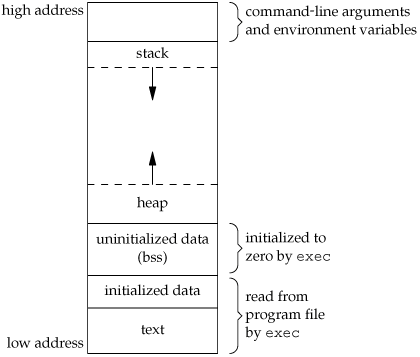
\includegraphics[scale=0.4]{images/memory-layout.png}\newline
    \caption{Agencement de la mémoire.}
\end{figure}


\myparagraph{Allocation et Libération: base des algorithmes}
\subparagraph{Allocation sur le tas}
Une des fonctions les plus connues des programmeurs et ingénieurs sous environnement UNIX est \textbf{malloc()} (respectivement \textbf{HeapAlloc()} sur
environnement Windows). En effet, en espace utilisateur, cette fonction est la base de l'allocation mémoire dynamique. Comme beaucoup de fonctions
manipulant le système d'exploitation et l'architecture sous-jacente, \textbf{malloc()} conserve son état tout au long de l'exécution et répertorie les
changements dans des données réservées à son utilisation (première zone libre, pointeurs sur une structure de base, etc...).
\subparagraph{}
Il existe de nombreuses alternatives au classique \textbf{malloc()}, provenant de bibliothèques externes et permettant de s'adapter aux besoins, voir d'améliorer les
performances globales (\textbf{gmalloc()}, \textbf{TCmalloc()}). Néanmoins, la base de l'algorithme reste le même quelle que soit la bibliothèque utilisée.

\subparagraph{Découpage en blocs du tas}
Pour gérer les allocations de différentes tailles, l'allocateur mémoire découpe au fur et à mesure des demandes
le segment qui lui est réservé. Ce découpage donne formation à des blocs mémoires qui sont marqués comme libre ou alloué, en gardant leur taille respective
en information.
\subparagraph{}
\begin{figure}
    \centering
    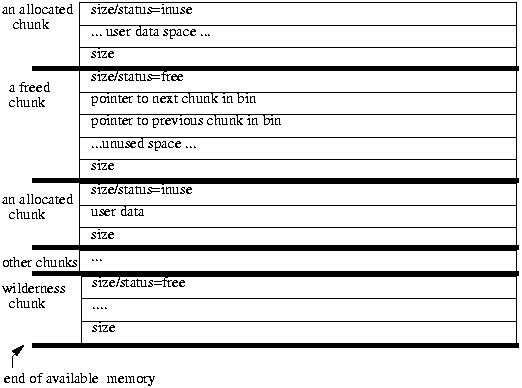
\includegraphics[scale=0.5]{images/malloc.png}\newline
    \caption{Implémentation basique de malloc.}
    \label{fig:malloc}
\end{figure}
Pour plus de rapidité lors de l'allocation et la libération, des liens sont conservés entre les différents blocs libres (suivant et précédent). Ainsi lors d'une allocation,
un parcours simple à partir du premier bloc libre permet de trouver un espace convenant à la demande. D'autres informations peuvent être stockées selon l'implémentation.
Un des exemples le plus courant est décrit dans la figure \ref{fig:malloc}\footnote{http://gee.cs.oswego.edu/dl/html/malloc.html}:

On remarque l'optimisation de l'espace pour les blocs libres. Au lieu d'utiliser de l'espace dans le cas général, qui ne servirait pas dans le cas des blocs alloués,
on préfère placer les pointeurs vers les autres blocs libres à l'intérieur de l'espace libre. Cela amènera d'ailleurs une discussion sur la granularité des allocations dans
les prochains paragraphes.
\subparagraph{}
La taille est également stockée au début et à la fin d'un bloc. Cela permet une coalescion plus simple des blocs libres. En effet quand deux blocs contigus en
mémoire sont libres, il est possible de les réunir en un seul plus gros blocs.

\subparagraph{Optimisation : cache}
Cette algorithme a cependant des limites. Si la fréquence d'allocation est rapide, et si les tailles allouées/libérées sont très variées, on retrouve un phénomène de
fragmentation important, et les blocs libres restant peuvent être trop petits pour une prochaine allocation, même s'ils auraient pu collectivement suffire.
\subparagraph{}
Pour assurer une fragmentation moins importante, la plupart des systèmes d'exploitation ont mis au point un système de cache (look-aside lists puis Low Fragmentation Heap sur Windows, différents sur Linux).
Le principe est simple : l'allocateur garde une liste des blocs libres d'une certaines taille. Selon l'algorithme utilisé, les tailles pré allouées peuvent différer.
On peut découper ces stratégies de caches en deux: la refonte différée et la pré-allocation.

\subparagraph{Refonte différée}
Au lieu de faire une refonte des blocs contigus lors de la libération, les blocs sont conservés libres et indépendants, et rajoutés à la liste des blocs libres de
la taille correspondante. Cela dans l'espoir que les prochaines allocations utiliseront une taille proche.

\subparagraph{Pré-Allocation}
Plutôt que d'attendre une libération, une partie de la mémoire initiale est pré-découpée pour remplir les caches. L'autre partie est conservée pour les allocations
ne rentrant pas dans les catégories mises en cache.

\subparagraph{}
Ce principe de cache est notamment très utile dans les environnements où la même taille est allouée un très grand nombre de fois. On peut imaginer par exemple un
algorithme allouant une structure pour chacun des utilisateurs s'enregistrant sur une application, ou simplement un service allouant la même taille un très grand nombre
de fois pour y stocker des messages. En termes de statistique, un programme a souvent un spectre de taille d'allocation réduit, ce qui a conduit à la présence systématique de
caches dans les algorithmes d'allocation mémoire.


\subparagraph{Granularité des allocations}
Comme évoqué précédemment, la granularité des blocs alloués peut varier selon les méthodes et les allocateurs utilisés. La "granularité" d'une allocation
correspond à une taille fixe dont la taille d'une allocation sera un multiple. En effet, même si l'utilisateur demande un bloc de 4 octets par exemple, la plupart
des allocateurs renverront un pointeur vers une zone allouée plus grande. Cela vient de plusieurs facteurs.

\subparagraph{}
Le premier concerne les méta-données conservées à l'intérieur ou autour du bloc alloué. Comme vu dans le schéma sur le découpage classique d'un bloc mémoire,
on retrouve plusieurs informations (comme des pointeurs en cas de blocs libres) à l'intérieur de la zone mémoire selon son état. Sur une architecture 64 bits,
deux pointeurs représentent en tout 16 octets. Ainsi, sans compter les méta-données entourant la zone mémoire réservée à l'utilisateur, une demande de blocs de taille
inférieure à 16 octets sera tout simplement arrondie.
\subparagraph{}
Sur Windows ou UNIX, les appels aux allocateurs courant sont souvent reliés intrinsèquement aux fonctions d'allocation plus "générales" comme  \textbf{VirtualAlloc()} sur
Windows, ou \textbf{sbrk()} et \textbf{mmap()} sur UNIX. Ces fonctions ont souvent une granularité beaucoup plus grande (64 kilo octets pour \textbf{VirtualAlloc()}, 4 kilo octets
pour \textbf{mmap()}). Les allocateurs mémoires ont pour but de gérer intelligemment et de manière transparente cet espace mémoire souvent trop gros pour une simple demande.

\subparagraph{Lien avec les vulnérabilités de type Use-After-Free}
Les optimisations présentées ci-dessus, bien qu'implémentées différemment selon les systèmes et bibliothèques, ont toutes un point commun.
Implémentées naïvement, elles augmentent certes la rapidité d'exécution, mais ceci au prix d'un déterminisme quasi-complet des zones allouées.
Une des conditions de base pour l'exploitation des vulnérabilités de type Use-After-Free est de pouvoir allouer la même zone mémoire que celle libérée plus tôt par le programme.
Le mécanisme de cache rend ceci beaucoup plus facile que si les zones étaient complètement aléatoires.

\subparagraph{}
Plusieurs implémentations ont été modifiées pour palier cet effet déterministe, et de nouveaux mécanismes de libération mémoire ont également vu le jour.
MemoryProtector, sur Windows, permet par le biais de la fonction \textbf{ProtectedFree()} de ne réellement libérer la mémoire que lorsque plus aucun pointeur
résidant sur la pile du programme ne pointe à l'intérieur de la zone mémoire ciblée.\footnote{http://community.hpe.com/t5/Security-Research/Efficacy-of-MemoryProtection-against-use-after-free/ba-p/6556134\#.VuEzVEL8tpg}


\subparagraph{}
Le sujet de stage porte toutefois sur la découverte d'une vulnérabilité en elle-même, et non pas sur son exploitation selon
le système d'exploitation, l'allocateur, etc.

\section{Moteur d'exécution symbolique}
\myparagraph{La finalité de l'exécution symbolique}
Un des défauts de l'analyse statique est l'absence de valeurs concrètes facilitant l'analyse. Même si c'est également
le but majeur de ce type d'analyse (la possibilité d'explorer tous les chemins), il est toujours agréable de conserver une valeur
associée à un identifiant ou à une zone mémoire, que ce soit sur la pile, sur le tas, ou dans d'autres segments. On peut ainsi se baser
sur ses valeurs pour évaluer les conditions pour prendre tel ou tel chemin, de réaliser des calculs, ou d'avoir tout simplement une référence en
matière de debug.
\myparagraph{Les bases de l'exécution symbolique}
Ce principe d'associer une valeur non-concrète à un identifiant ou une zone mémoire est connu sous le nom d'exécution symbolique. Comme son nom
l'indique, le principe est d'initialiser la valeur à un symbole lorsqu'elle est créée, et d'exécuter le programme en se basant sur cette valeur initiale.
Par exemple, sur x86, le registre \textbf{EAX} pourra être initialisée à la valeur \textbf{EAX\_INIT}. Ainsi une future opération \textbf{add EAX, 4} assignera
au même registre la valeur symbolique \textbf{EAX\_INIT + 4}.

\subparagraph{}
Un moteur d'exécution symbolique complet contiendra également les opérations classiques en programmation, comme le déréférencement mémoire d'une valeur
symbolique, les opérations arithmétiques, etc. Concernant les opérations liées à la mémoire, la plupart des moteurs choisissent de créer un espace associé à
un espace mémoire concret uniquement lorsque celui-ci est adressé en écriture. Cela permet de garder une double dimension début/taille sans pourtant autant
nécessiter une représentation excessivement volumineuse en termes de mémoire par l'outil.
\subparagraph{}
Cela peut néanmoins poser problème si le programme essaye d'accéder à une
zone non initialisée (ce qui peut être une vulnérabilité en soit pour un programme). Soit l'outil utilisé peut rencontrer un problème et terminer en erreur,
ou retourner une valeur nulle. Dans certains cas d'analyse, on peut néanmoins tout simplement initialiser la mémoire si celle-ci ne l'était pas déjà à une valeur concrète
par défaut ou bien à un symbole non utilisé ailleurs.

\myparagraph{Concolique: un mélange de concret et de symbolique}
Prenons l'exemple de la figure \ref{fig:condition} pour illustrer le principe de l'exécution concolique. Deux chemins sont possibles: l'un menant à un appel à \textbf{g()}, l'autre à \textbf{h()}.
\begin{figure}[h]
    \centering
    \begin {lstlisting}[frame=single]
int main(void)
{
    int a = f();
    if (a == 0)
        g();
    else
        h();
}
    \end{lstlisting}
    \caption{Branchement restrictif à une seule valeur.}
    \label{fig:condition}
\end{figure}
L'analyse peut alors se séparer en deux chemins. Néanmoins, pour le chemin menant à \textbf{g()}, la valeur de l'identifiant \textbf{a}
n'a qu'une seule possibilité, la valeur 0. Certains solveurs de contraintes, dont nous parlerons dans la prochaine section, permettent d'arriver
à des conclusions comme celle ci en gardant toutes les contraintes valables pour un chemin.
\subparagraph{}
Dans des cas comme celui-ci, la valeur est directement injectée dans le moteur d'exécution symbolique. Ce mélange de valeur concrète et symbolique est
appelé \textbf{exécution concolique}. Cela permet de réduire le temps de calcul des assertions (la valeur correspondante étant déjà prise en compte) et de
réduire en mémoire la taille des expressions symboliques.


\section{Solveurs SMT}
\myparagraph{Contraintes associées aux chemins}
Dans un programme, une division de l'analyse en deux est toujours dûe à la même structure : une condition liée à une boucle ou à une structure de type if-then-else.
Cette condition sur une valeur donnée réduit (à moins que la condition ne soit sémantiquement pas correcte initialement) le champs de valeur possible pour un identifiant.
Parfois même, la condition ou l'enchainement des conditions sur un même chemin d'exécution est assez restrictive pour ne donner qu'une seule valeur possible.
Même si cela peut paraitre évident pour une analyse manuelle, il peut être délicat de résoudre ces contraintes sans aide extérieure. C'est donc le but de ce qu'on appelle : les \textbf{solveurs SMT}.
\subparagraph{}
Un \textbf{solveur SMT} (Satisfiabilité Modulo Théories) permet de résoudre un ensemble de contraintes exprimées dans la logique du premier ordre. Ce type de solveur peut décider
de la solvabilité ou non de cet ensemble de contraintes. Cela permet, par exemple lors de l'analyse statique, de ne pas prendre un chemin dont les valeurs associées n'auraient
de sens d'un point de vue relationnel.
\subparagraph{}
Pour un chemin dont les contraintes sont satisfaisables selon le solveur SMT, ce même solveur peut fournir un modèle. Ce dernier représente l'ensemble des valeurs possibles
pour les variables rentrant en jeu dans les contraintes. Lorsque plusieurs valeurs sont possibles, on peut au choix et selon le but de l'analyse, sauvegarder les contraintes
en espérant de futures conditions plus restrictives, ou assigner un des ensembles de valeurs à nos identifiants symboliques.
\subparagraph{}
Dans l'exemple \ref{fig:condition}, les contraintes du solveur serait (en utilisant la représentation intermédiaire de Miasm):
\begin{itemize}
    \item ExprId('a') == 0 lors de l'appel à g. Le seul modèle possible est [ a == 0].
    \item ExprId('a') != 0 lors de l'appel à h. Un des modèle possible est [ a == 1 ].
\end{itemize}



\section{Choix d'implémentation: outils de décompilation}
\myparagraph{Critères de sélection}
Pour réaliser le sujet de stage, en dehors du langage de programmation en lui-même, un ou plusieurs outils effectuant
un pré-traitement sur l'entrée était nécessaire. En effet, la solution finale prend en entrée un programme binaire et un point
d'entrée. Il n'était pas concevable d'effectuer le traitement sur du binaire, ou d'effectuer une analyse différente selon le format
et l'architecture visée par le binaire (les instructions étant différentes).
\subparagraph{}
Un moteur d'exécution symbolique est également de mise. Il représente à lui seul une grosse partie de l'analyse statique permettant de
garder en mémoire les valeurs des identifiants par rapport à leur valeur d'origine. Un solveur SMT permet également de réduire le nombre
de chemins possibles et réduit souvent drastiquement le problème d'explosion de chemins.
\subparagraph{}
Il a donc fallu chercher un ou plusieurs outils de base, pouvant effectuer la décompilation du binaire puis la transformation en une
représentation intermédiaire. Heureusement, la plupart des outils libres d'analyses binaires proposent les deux, souvent de manière transparente.
Ils proposent également leur moteur d'exécution concolique associé. Le solveur SMT est la plupart du temps imposé. En effet, ce type de solveur prend
en entrée une syntaxe et des objets particuliers, qu'il faut traduire. Ainsi la traduction de la représentation intermédiaire est intrinsèquement liée à cette
représentation, et re-coder une traduction de chaque objet pour un solveur particulier prendrait trop de temps pour être rentable sur la durée d'un stage.
\subparagraph{}
Les outils consultés feront chacun l'objet d'un chapitre, et le choix final ainsi que les comparaisons faites seront résumées à la fin.

\myparagraph{Angr}
\begin{figure}[h]
    \centering
    
\includegraphics[scale=0.3]{images/angr.png}
    \caption{Logo d'Anr.}
\end{figure}
Angr\footnote{https://github.com/angr/pyvex} est un projet d'analyse binaire créé par le laboratoire de sécurité informatique de l'UC Santa Barbara (USA).
Il permet de charger un binaire et d'avoir une représentation de celui-ci en utilisant un langage intermédiaire intermédiaire, \textbf{VEX}.
Il dispose également d'un moteur d'exécution symbolique et est très complet dans ses fonctionnalités, permettant de récupérer une certaine quantité d'information via
une API plutôt complète. La résolution des contraintes est réalisée grâce à un module interne nommé \textbf{Claripy}
\subparagraph{}
En termes de maturité, le projet a vite atteint une autre dimension, et ses utilisateurs sont de plus en plus nombreux. Il supporte plusieurs formats
binaire (PE, ELF, IdaBin, ...) ainsi que la plupart des architectures classiques (AMD64, MIPS, ARM, ...).

\myparagraph{Miasm}
\begin{figure}[h]
    \centering
    
\includegraphics[scale=0.3]{images/cea.png}
    \caption{Logo du CEA.}
\end{figure}
Miasm\footnote{https://github.com/cea-sec/miasm} est un projet développé principalement par des membres de l'équipe IT Security du Comité à l'Energie Atomique (CEA).
Il dispose de toutes les fonctionnalités nécessaires (moteurs d'exécution, etc.). Il supporte également les architectures courantes. Le solveur de contraintes est
cependant externe, l'outil traduisant juste la représentation intermédiaire vers un langage compréhensible par le très connu Z3 de Microsoft.
\subparagraph{}
Un des inconvénients de Miasm est ses fortes dépendances envers un nombre élevé de bibliothèques externes, sur des versions parfois obsolètes. La documentation est également
quasi-inexistante.
\newpage
\myparagraph{Capstone}
\begin{figure}[h]
    \centering
    
\includegraphics[scale=0.3]{images/capstone.png}
    \caption{Logo du Capstone.}
\end{figure}
\begin{center}
\end{center}
Capstone\footnote{http://www.capstone-engine.org/} est la star montante du monde de la rétro-ingénierie. En plus d'une communauté gigantesque et d'une
documentation bien construite, de nombreux projets se basent déjà sur son architecture. De plus, le projet est plutôt jeune, ce qui permet d'avoir des
dépendances récentes. La plupart des distributions ont de toute manière des paquets déjà prêts pour une installation simplifiée.
\subparagraph{}
Néanmoins, aucune représentation intermédiaire n'est directement proposée par l'infrastructure de Capstone (même si plusieurs projets comme OpenReil se sont basés
dessus pour fournir une représentation intermédiaire).


\myparagraph{Comparaison}

\begin{table}[h]
    \centering
    \caption{Comparatif des suites de rétro-ingéniérie/analyse choisies}
    \label{itd}
    \begin{tabular}{c|c|c|c}
                      & Angr     & Miasm   & Capstone \\
        \hline
        Graphe        & Oui      & Oui     & Non      \\
        \hline
        RI            & Oui      & Oui     & Non      \\
        \hline
        Documentation & Oui      & Non     & Oui+     \\
        \hline
        Connu         & Oui      & Oui     & Oui+     \\
        \hline
        Plateforme    & x86,MIPS & x86,ARM & A lot
    \end{tabular}
\end{table}

Au moment de cette réflexion, Angr n'avait pas vraiment été
considéré (ce qui sera d'ailleurs marqué comme une erreur plus tard lors du bilan du stage).
Miasm permettant de faire tout ce qui avait été établi lors du cahier des charges, c'est donc cette suite d'outils qui fut choisie.
Même si la documentation lui fait cruellement défaut, la plupart des exemples suffisent à prendre en main (de manière basique) l'ensemble.
\subparagraph{}
Une étude plus en profondeur de l'outil a ensuite aidé à mieux affiner son usage et à utiliser des fonctions internes pour réaliser des travaux
plus finement.

\section{L'analyse statique d'Use-After-Free}
\myparagraph{Graphe d'instructions}
Le graphe d'instructions d'un programme est représenté sous la forme d'un graphe orienté dont les nœuds rassemblent une ou plusieurs
instructions (intermédiaires ou liées à l'architecture). Les arcs de ce graphe relient les instructions dans leur ordre d'exécution.
Un nœud peut avoir un ou plusieurs arcs entrants, ainsi que un ou deux arcs sortants (dans le cas d'une condition par exemple).
\begin{figure}[h]
    \centering
    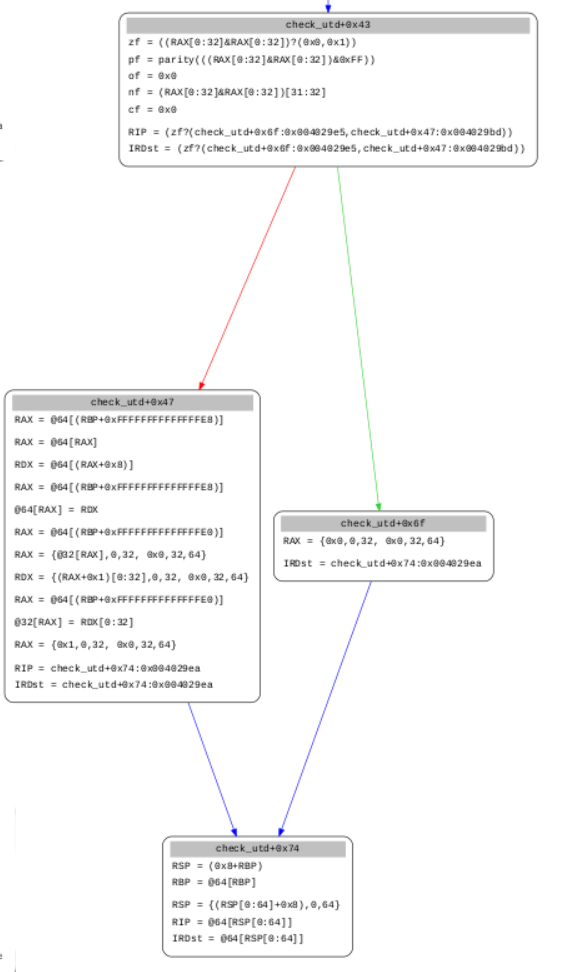
\includegraphics[scale=0.3]{images/condition.png}\newline
    \caption{Exemple de graphe avec conditions.}
    \label{fig:graph-cond}
\end{figure}
\subparagraph{}
L'illustration \ref{fig:graph-cond} est la représentation graphique d'un exemple de graphe qui sera parcouru durant l'analyse. Le graphe est parcouru \textbf{dans l'ordre},
en partant d'un point d'entrée donné. Ce \textbf{point d'entrée} peut soit être \textbf{une adresse en hexadécimal} (0xABCDF) ou \textbf{un nom de fonction
suivi possiblement d'un offset hexadécimal} (main[+0x12]). Cette entrée doit correspondre à un \textbf{label} présent sur un des nœuds du graphes.
\subparagraph{}
Durant la décompilation, Miasm découpe le programme en \textbf{\textit{basic blocks}}. Un \textit{basic blocks} est défini comme ceci :
une suite d'instruction successives se terminant par un branchement ou un point de sortie. Cela permet de découper en fonction logique
le programme et de le représenter sous forme de diagramme de décision. La lecture est alors plus simple, plus naturelle, et les chemins se suivent et se
séparent logiquement, ressemblant plus à la manière dont le code source se divise que celle du code binaire/assembleur.
\subparagraph{}
Miasm génère également d'autres \textbf{basic blocks} lors des appels de fonctions. Ils permettent de traiter différemment ces blocs, d'effectuer une pré-analyse
de la fonction, etc.

\myparagraph{Representation intermédiaire de Miasm}
Toutes les instructions de la représentation intermédiaire de Miasm sont représentées sous la forme d'une assignation : EXPR1 = EXPR2.
L'expression de gauche étant un registre ou un espace mémoire valide, et l'expression de droite pouvant être n'importe quelle expression
représentant in fine une valeur.
\subparagraph{}
En interne, les expressions sont découpées en 5 types, tous défini par une taille (généralement 32 ou 64 bits) et des arguments optionnels:
\begin{itemize}
    \item Les ExprInt : un entier, d'une taille définie.
    \item Les ExprID : un identifiant, le plus souvent un registre.
    \item Les ExprMem : un espace mémoire, dont l'adresse est donnée par l'argument de l'expression. Cette expression peut être de n'importe quel type.
    \item Les ExprOp : une opération entre deux expressions (les opérations mathématiques classiques ainsi que les appels de fonctions).
    \item Les ExprCond : une condition. La condition est représentée par une expression selon le même principe qu'en C. Si la valeur de l'expression est 0, la condition est fausse,
sinon elle est considérée comme vraie. Une ExprCond prend également en paramètre deux expressions représentant le branchement à prendre (souvent des ExprInt.
    \item les ExprSlice et ExprComp : composition et décomposition d'un ou plusieurs emplacements selon un nombre de bits précis.
\end{itemize}
En prenant en exemple le graphe suivant, un début de lecture serait le suivant:
\begin{itemize}
    \item Pour le \textit{basic block} \textbf{main+0x23}, la première instruction (\textbf{ExprMem}) assigne à l'emplacement désigné par \textbf{l'adresse}
        présente dans \textbf{ESP} la valeur \textbf{0x4}.
    \item Les blocs se finissent tous par une assignation de l'identifiant \textbf{IRDst}, indiquant le prochain basic bloc dans l'exécution.
        En l'occurence, toutes les assignations de cet exemple sont des \textbf{ExprInt}). S'il s'agissait d'un branchement, l'expression assigné à \textbf{IRDst}
        aurait été de type \textbf{ExprCond}.
\end{itemize}
\begin{figure}[h]
    \centering
    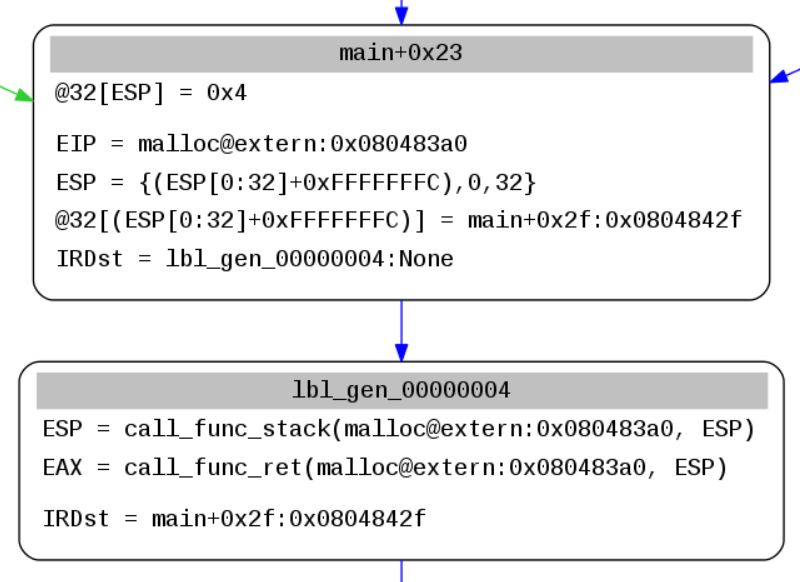
\includegraphics[scale=0.3]{images/ir.png}\newline
    \caption{Représentation intermédiaire d'un appel de fonction.}
\end{figure}
\subparagraph{}
Chacune des instructions intermédiaires représente une ou plusieurs instructions du binaire ciblé. En effet, un langage intermédiaire
pouvant se retrouver à travailler sur plusieurs architectures cibles, une instruction complexe sur une d'elle est retransformée en de multiples
fragments, pouvant alors se retransformer/ré-assembler sur une autre architecture si besoin.
\subparagraph{}
Chacun des \textit{basic blocks} est divisé en "déclaration". Ces déclarations réunissent des instructions qui effectuent une même action. Une instruction cible décomposée
verra sa transformation, possiblement constituée de plusieurs instructions intermédiaires, regroupée en une seule "déclaration".



\myparagraph{Reconnaitre un use-after-free}
Comme dit précédemment, un use-after-free est l'enchainement d'une allocation, d'une libération, puis de l'utilisation d'un espace mémoire.
\subparagraph{Allocation}
Une \textbf{allocation} dans le sens de la présente analyse, est l'appel d'une fonction étant marquée comme \textit{allocatrice}. En reprenant les deux noeuds intermédiaires
du paragraphe précédent, on peut comprendre comment Miasm traduit un appel de fonction. Dans le cas présenté, il s'agissait d'une allocation en utilisant la fonction malloc,
avec comme argument la taille d'une zone de stockage de type C \textbf{int}.
Le registre d'instruction (ici \textbf{EIP}) est mis à jour, les arguments sont placés dans les registres qui conviennent ou bien sur la pile.
Ici \textbf{0x4} est poussé sur la pile. Le binaire décompilé étant conçu pour l'architecture x86, \textbf{ESP} est également décrémenté de \textbf{4 octets},
et l'adresse de la prochaine instruction est stockée sur la pile.
\subparagraph{}
Miasm génère alors un \textit{basic block} virtuel (\textit{lbl\_gen\_X}) qui stocke la valeur de retour de la fonction (\textbf{ExrOp(call\_func\_ret)})
là où la convention d'appel du binaire le veut. Le principe suivant est appliqué:
\begin{enumerate}
    \item La fonction est-elle annotée \textbf{@extern} ? Si non, l'analyse continue en suivant cet appel.
    \item La fonction est-elle marquée comme allocatrice ? Si oui, la valeur de retour ainsi que le registre servant à la stocker sont mémorisés.
\end{enumerate}

\subparagraph{Libération}
En suivant le même principe que pour l'allocation, si une fonction est marquée comme libératrice, si ses arguments sont mémorisés comme faisant référence
à une zone mémoire précédemment allouée, cette zone est marquée comme libre.

\subparagraph{Utilisation}
Lors du parcours du graphe, lorsqu'une instruction intermédiaire est analysée, si la source comprend une référence à une zone mémoire marquée comme libre,
un UAF est détecté.

\myparagraph{Algorithme basique}
L'exemple de pseudo-code de la figure \ref{fig:analyse} illustre l'algorithme utilisé pour la base de l'analyse.
\newpage
\begin{figure}[h!]
    \centering
    \begin {lstlisting}[frame=single]
allocation_id = 0
head_node = flowgraph.get_node(start)

ir_block = ir.get_bloc(head_node)
for statement in ir_block:

    evaluate_ir(statement)

    for dst, src in statement:

        check_if_src_depends_on_free(free_set, src)

        # Propagate tainted expression
        del tracking_set[dst]
        if src in tracking_set:
            tracking_set[dst] = tracking_set[src]

        if src.is_function_call() and "ret" in str(src):
            # If alloc_tracking_set, track the newly
            # allocated memory address
            if call_name in allocation_functions:
                tracking_set[dst] = allocation_id
                allocation_id = allocation_id + 1

            # If free_tracking_set, mark the
            # corresponding zone as free
            if call_name in free_functions:
                free_set.add(tracking_set[arguments])

go_to_next_basic_block()
    \end{lstlisting}
    \caption{Squelette d'analyse Use-After-Free.}
    \label{fig:analyse}
\end{figure}

L'algorithme utilise deux structures de données très importantes :

\begin{itemize}
        \item tracking\_set : un dictionnaire associant un identifiant ou une zone mémoire à un identifiant d'allocation.
        \item free\_set : un ensemble des identifiants d'allocations libérés.
\end{itemize}

Chaque allocation se voit attribuer un identifiant unique (\textbf{allocation\_id}). Cela permet de centraliser les informations
en utilisant uniquement cet identifiant lorsque nécessaire.

L'algorithme ci-dessus est du pseudo-code sur un traitement simple.
Premièrement, le nœud courant (\textit{basic block}) est récupéré du graphe. Pour chaque instructions du graphe, on évalue symboliquement
l'expression afin de mettre à jour le moteur d'exécution symbolique.
\subparagraph{}
L'expression source est vérifiée afin de s'assurer qu'elle ne dépend pas d'un bloc mémoire libéré.
\subparagraph{}
Ensuite, on supprime (si présente) la destination de l'assignation de l'ensemble d'expressions traquées. En effet, celle ci va prendre une nouvelle valeur et est donc
réinitialisée. Si la source dépend d'un bloc connu, on met à jour le dictionnaire.
\subparagraph{}
Selon la fonction appelée, on peut soit ajouter un nouveau bloc, soit en libérer un, soit ne rien faire.
\myparagraph{Teinte}
Ce principe de teinte est excessivement utilisé dans l'analyse de binaire ou de programme. Le principe est simple, intuitif et plutôt modulaire selon l'analyse, il n'y aura
donc pas d'explication détaillée de son fonctionnement dans ce rapport. Néanmoins les notions de base sont les suivantes:
\begin{itemize}
        \item Un élément de l'analyse est marqué comme teinté lors d'une procédure définie.
        \item Lorsque cet élément est en contact ou lié avec un autre élément, et que cette liaison respecte certains
            critères, cet autre élément est également marqué comme teinté.
        \item Chaque teinte doit avoir une couleur. La couleur est possiblement la même pour chaque élément teinté.
\end{itemize}

\myparagraph{Architecture du scanner et objets}
Le but de tout projet à long terme est d'être maintenable par des nouveaux arrivants, et de pouvoir s'améliorer
sans difficultés. Cela passe par la documentation, mais également par une architecture et une conception réfléchie à l'avance
et si possible modulaire.
\newpage
\subparagraph{Architecture}
Le projet est divisé en trois parties:
\begin{enumerate}
        \item Le parcours de graphe
        \item L'analyse et le marquage (teinte)
        \item Les optimisations de parcours du graphe.
\end{enumerate}
Chaque couche X est plus ou moins dépendante de la couche X-1. Néanmoins, l'inverse ne doit pas être vrai.
Si l'analyse et le code associé commencent à dépendre de la manière dont l'optimisation évolue, alors la conception commence à poser problème.
En effet, si une optimisation prend le pas sur d'autres, on restreint les possibilités. Une phrase célèbre de Donald Knuth résume d'ailleurs cette situation:
\textit{L'optimisation prématurée est la racine de tous les maux}.
\subparagraph{}
\begin{figure}[h]
    \centering
    \begin {lstlisting}[frame=single]
allocation_id = 0
head_node = flowgraph.get_node(start)

ir_block = ir.get_bloc(head_node)
# Do something 1
for statement in ir_block:
    # Do something 2
    for dst, src in statement:
        # Do something X
        if src.is_function_call() and "ret" in str(src):
            # Do something Y
            if must_follow_function_call:
                follow_function_call()
        # Do something Z

go_to_next_basic_block()
    \end{lstlisting}
    \caption{Squelette de parcours de graphe.}
    \label{fig:graph-walk}
\end{figure}
Le parcours de graphe est en réalité un squelette, avec plusieurs endroits dans lesquels il est possible de faire des traitements ou optimisations. L'algorithme de base
épuré pour ne laisser que le parcours de graphe ressemble au code de la figure \ref{fig:graph-walk}
\newpage
\subparagraph{Modules python}
Le projet est découpé en plusieurs modules python:
\begin{itemize}
        \item Le scanner en lui même.
        \item Le "moteur" de teinte.
        \item Le module annexe contenant tous les algorithmes utiles (sur les graphes, factorisation de listes, etc.).
\end{itemize}

\subparagraph{L'objet Scanner}
Un scanner est représenté par un objet Python. Il contient plusieurs propriétés et méthodes permettant de le manipuler directement.
Les attributs principaux sont:
\begin{itemize}
    \item \textbf{disassemble\_callback} : Fonction à appeler pour aller récupérer un bloc dans un graphe.
    \item \textbf{alloc\_tracking\_set} : Ensemble de fonctions allocatrices de mémoire.
    \item \textbf{tracking\_set} : Dictionnaire reliant expressions et identifiants d'allocation.
    \item \textbf{free\_tracking\_set} : Ensemble de fonctions libératrices de mémoire.
    \item \textbf{free\_set} : Ensemble d'identifiants d'allocation libérés.
    \item \textbf{register\_var\_counter} : Compteur d'identifiant d'allocation
    \item \textbf{positive\_results} : Ensemble des chemins menant à une vulnérabilité répertoriée durant cette passe.
    \item \textbf{pre\_analyze} : Dictionnaire contenant différentes informations sur chacune des fonctions déjà visitées. \textit{Optimisation}.
    \item \textbf{stack\_arguments} : Arguments placés sur la pile jusque là.
    \item \textbf{marked} : Dictionnaire reliant les nœuds du graphe au nombre d'exécution symbolique de ce nœud sur un chemin. \textit{Optimisation}.
    \item \textbf{loop\_mark} : Dictionnaire reliant un nœud au \textbf{tracking\_set} lors de sa dernière visite. \textit{Optimisation}.
    \item \textbf{useless\_branches} : Dictionnaire reliant un nœud aux différents branchement qui n'ont aucune conséquence sur l'analyse. \textit{Optimisation}.
\end{itemize}
L'utilité et le fonctionnement des attributs avec la marque \textit{optimisation} seront expliqués dans une prochaine partie.
\subparagraph{}
L'objet scanner étant un objet qui sera souvent amené à être copié, les attributs sont réduits au minimum. Quand cela est possible, une passe est faite sur
ces attributs pour les factoriser. Par exemple, un attribut auxiliaire, \textbf{path}, qui désigne les nœuds actuellement parcourus sur le chemin, subit un traitement
à chaque ajout pour factoriser les boucles se répétant plus de deux fois.
\subparagraph{}
Pour des soucis de parallélisme, qui seront expliqués plus en détail par la suite, certains attributs ne peuvent pas être externalisés au scanner. Ils doivent faire partie
intégrante de l'objet pour garder leur état. Ceci pose un problème d'espace mémoire copié inutilement, mais il n'est malheureusement pas possible de faire autrement avec
la technique de parallélisme utilisé et le fonctionnement interne de Python. C'est par exemple le cas de \textbf{register\_var\_counter} qui devrait faire partie du moteur de teinte.

\myparagraph{Modification du comportement par défaut de Miasm}
Le désassemblage et l'exécution symbolique de Miasm fonctionne de manière plus ou moins satisfaisante dans la plupart des cas. Néanmoins,
certains comportements ne convenaient pas à l'analyse présentée dans ce rapport. Deux sont à noter: les appels de fonctions lors de l'exécution symbolique ainsi que
la récupération des symboles.
\subparagraph{Récupération des symboles}
Dans sa conception, Miasm utilise un autre projet, \textbf{Elfesteem}, qui permet d'extraire les informations de binaire de type PE ou ELF. Elfesteem permet notamment
de récupérer les sections (dossier/table) dans les formats ELF (PE). Les deux formats peuvent stocker des symboles, qui ne sont que des noms associés à une valeur.
Dans le cas des fonctions externes au programme, dans le format ELF par exemple, les sections \textbf{.symtab} et \textbf{.plt} permettent de faire la liaison entre un appel de fonction
externe et son adresse. Si les symboles internes sont également gardés lors de la compilation, on peut également les utiliser pour avoir une analyse plus claire et plus facile à interpréter lors
de déboguage.
\subparagraph{}
Cependant, Miasm n'annote pas le graphe avec les informations présentes dans le binaire. Il a donc été nécessaire de modifier le comportement lors du desassemblage afin que le graphe se construisent
en se basant sur ces données.

\subparagraph{Appels de fonction et exécution symbolique}
\begin{figure}[h]
    \centering
    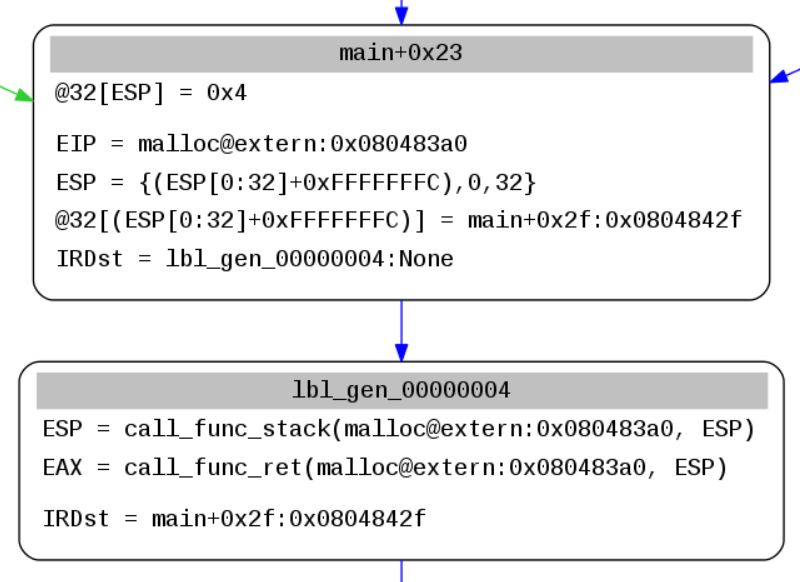
\includegraphics[scale=0.3]{images/ir.png}\newline
    \caption{Représentation intermédiaire d'un appel de fonction.}
\end{figure}
L'exécution symbolique est faite pour que l'abstraction se fasse automatiquement et que les valeurs soient constamment à jour sans travail nécessaire de la part de l'utilisateur. Avec les appels de
fonctions (notamment externes), plusieurs problèmes se posent.
\begin{itemize}
    \item Lors des instructions comme \textit{EAX = call\_func\_ret(...)}, EAX est automatiquement assigné à la valeur ExprOp(call\_func\_ret(...)). Si la fonction est interne et que
    son exécution est possible, EAX sera de toute manière bien assigné à une vraie valeur de retour. Le fait d'exécuter l'instruction donnée en exemple remplace cette bonne valeur par quelque
    chose d'imprécis.\newline
    Il suffit d'ignorer les instructions de ce genre si la fonction appelée est exécutable symboliquement (si sa representation intermédiaire est disponible).
    \item De la même manière l'instruction utilisant ESP peut conduire dans des situations non désirable. Lorsqu'une fonction est sur le point d'être appelée, Miasm effectue de lui même le décalage de la pile pour permettre de stocker le pointeur d'instruction de retour.\newline
    Néanmoins dans certaines conventions d'appel, c'est la fonction appelée et non la fonction appelante qui doit nettoyer la pile. Si la fonction est externe, le second décalage ne se fera donc pas et il faut alors l'effectuer à la main.
\end{itemize}

\myparagraph{Explosion de chemin et Optimisation de boucles}
Pour chaque branchement, l'analyse continue sur les branches dont la condition peut être satisfaisable (selon le solveur SMT). En x86 et dans la plupart des architectures,
un branchement ne peut mener qu'a deux endroits au maximum. Lors d'une boucle, une lecture simpliste pourrait mener à dire que le branchement de sortie ou d'entrée dans la boucle n'est présent qu'une fois.
\subparagraph{}
Pourtant, lors de l'exécution symbolique, à chaque fois que l'on rentre dans une boucle, ce branchement sera re-rencontré une autre fois, et ainsi de suite.
On remarque alors que l'analyse peut possiblement se diviser indéfiniment en deux, menant ainsi à ce qu'on appelle une \textit{explosion de chemins}.
\subparagraph{}
Pour palier à ce problème, tout en gardant une analyse correcte, il faut trouver un moyen d'éviter de parcourir une boucle lorsque ceci est inutile. Cela est possible grâce à plusieurs heuristiques:
\begin{itemize}
    \item Le \textbf{tracking\_set} du scanner n'a pas changé depuis son dernier passage, l'analyse devient invariante.
    \item Le nœud suivant sur la branche a déjà été exécuté un nombre excessif de fois dans le contexte courant (dans la même boucle).
    \item La boucle courante est une boucle infinie volontaire (par exemple un serveur recevant les demandes de clients). On peut quitter l'analyse au bout d'un certain temps.
\end{itemize}
\subparagraph{}
\begin{figure}[h!]
    \centering
    \begin {lstlisting}[frame=single]
# Si le bloc a deja et visite
if start in scanner.marked:
    if scanner.marked[start] > LIMIT_VISIT_NODE:
        return
    # Si le bloc est deja marque comme present dans
    # une boucle
    if start in scanner.loop_mark:
        # Si la derniere analyse a produit le meme
        # contexte que la passe courante
        start_mark = scanner.loop_mark[start]
        if start_mark == scanner.tracking_set:
            # On recupere le noeud precedent et on
            # precise que le branchement entre ce noeud
            # et le noeud courant est devenu inutile
            prev = previous(start)
            scanner.useless_branches[prev].add(start)

    [...]

if next not in scanner.useless_branches[start]
        and not in_infinite_loop(start):
    go_to_next_basic_block()
    \end{lstlisting}
    \caption{Optimisation de boucles.}
    \label{fig:fix-point}
\end{figure}
L'algorithme \ref{fig:fix-point} essaye de déterminer un \textit{point fixe} dans l'analyse. C'est à dire que ré appliquer l'analyse avec le contexte courant sur cette branche serait
égal à ce qui a déjà été fait.

Sans ces heuristiques là, l'analyse est quasi certaine de boucler indéfiniment. La comparaison du contexte dans le pseudo-code est également simplifiée pour des soucis de lisibilité.
Imaginons que l'analyse passe dans une boucle où un objet est alloué, utilisé, puis supprimé (un envoie de message sur le réseau par exemple). Les deux contextes
ne seront pas strictement égaux. C'est à dire que les identifiants d'allocation contenus dans les mêmes zones mémoire seront décalés.
\subparagraph{}
\newpage
On peut prendre en compte ce phénomène en ne prenant pas uniquement en compte les identifiants d'allocations, mais également une possible \textit{traduction}:
\begin{enumerate}
    \item On vérifie que l'on retrouve les mêmes éléments teintés dans les deux contextes c1 et c2.
    \item Pour chaque élément dans c1, on regarde si l'identifiant d'allocation i1 dans c2 est le même i2 (i1 == i2), si oui, on passe au suivant.
    \item Si non, on vérifie que tous les éléments teintés dans c1 avec le même identifiant i1 ai la même traduction i2 dans c2.
\end{enumerate}
\subparagraph{}
Certains identifiants ne sont également pas pris en compte dans la comparaison. En effet, le registre contenant la valeur de retour d'une fonction peut gêner la comparaison
lorsqu'il est assigné en fin de boucle. Les drapeaux (\textbf{EFLAGS}) sont également non compris dans toute l'analyse (la durée entre leur assignation et leur utilisation étant généralement d'une
ou deux instructions machine).


\myparagraph{Appel de fonctions}
Lorsqu'une fonction est appelée, le scanner lance l'analyse avec le contexte courant sur le premier nœud de cette fonction. Comme une analyse classique, celle de la fonction peut se diviser
en plusieurs lorsqu'un branchement est rencontré. On se retrouve donc possiblement avec plusieurs chemins retournant de cette fonction. Afin de différencier chacun de ces chemins (et donc contexte),
un appel à une fonction accumule les retours de l'analyse. Une fois tous les retours obtenus, tous les contextes retournant sont lancé sur le nœud suivant.
\begin{figure}[h]
    \centering
    \begin {lstlisting}[frame=single]
void g(int *a)
{
    // g1
    if (*a == 3)
    // g2
    *a = 4;
    else
    // g3
    *a = 3;
}

void f(void)
{
    // f1
    int a = rand();
    g(&a);
    if (a == 3)
    // f2
    puts("a == 3");
    else
    // f3
    puts("a != 3");
}
    \end{lstlisting}
    \caption{Exemple d'explosions de chemin.}
    \label{fig:path-explosion}
\end{figure}
Dans l'exemple \ref{fig:path-explosion}:
\begin{enumerate}
    \item le chemin f1-() appele g()
    \item le chemin f1-g1-() se sépare en deux.
    \item En retour de g(), deux chemins et contextes sont retournés :
    \begin{itemize}
        \item f1-g1-g2-()
        \item f1-g1-g3-()
    \end{itemize}
    \item Ces deux chemins continuent leurs analyses. Le branchement crée donc :
            \begin{itemize}
                \item f1-g1-g2-f2-()
                \item f1-g1-g2-f3-()
                \item f1-g1-g3-f2-()
                \item f1-g1-g3-f3-()
            \end{itemize}
\end{enumerate}
Possiblement, plusieurs contextes retournés par une fonction seront égaux. Si cela est le cas,
ces cas là sont rassemblés en un seul pour éviter de l'encombrement spatial et temporel inutile.

\myparagraph{Pre-Analyse}
Comme vu au chapitre précédent, appeler une fonction peut être lourd pour le traitement. Optimiser le retour
ou l'appel de ces fonctions est primordial pour éviter d'utiliser trop de ressource ou bien pour raccourcir la durée de traitement.
Concernant l'appel, une question simple permet d'optimiser rapidement l'ensemble: est-ce qu'appeler cette fonction aura un impact sur le contexte courant.

\subparagraph{}
Une fonction peut possiblement modifier le contexte si:
\begin{itemize}
    \item Elle contient un appel à une fonction allocatrice.
    \item Elle contient un appel à une fonction libératrice.
    \item Elle modifie une variable globale possiblement teintée.
\end{itemize}
Une pre-analyse ressemble fortement à l'analyse concrète présentée plus tôt, à ceci près qu'aucune exécution symbolique n'est faite, aucune information n'est stockée
tout au long du chemin. Une fois qu'un des trois critères est rencontré, la pre-analyse se termine directement et son résultat est retourné.
Si un appel de fonction a lieu durant la pre-analyse, la fonction appelée est pré-analysée à son tour, etc.
\subparagraph{}
Ces informations ne changent pas selon le contexte, par conséquent, ces résultats peuvent être stockés globalement et utilisés par tous les objets scannés
durant leurs analyses. Néanmoins, pre-analyser toutes les fonctions au lancement de l'outil peut être très consommateur, et possiblement inutile. En conséquence,
ce principe est soumis à ce qu'on appelle l'\textit{évaluation feignante} (\textit{lazy evaluation}). Une fonction n'est pré-analysée que lorsqu'elle est appelée pour la première fois.
Une fois cette pre-analyse faite, le pilote, gouvernant tous les chemins, stocke le résultat, et le transmet au prochain chemin en cours d'analyse. Ce principe permet de garder une base
commune et légère au possible.

\myparagraph{Traitement parallèle ou continu}
Comme dit plusieurs fois auparavant, une analyse peut se diviser. Chacune de ses divisions crée un nouveau travail (job). Ces travaux sont stockés dans une file d'attente
puis exécutés. Le problème reste à savoir si plusieurs analyses auront lieu en même temps ou non. Plus le nombre travaux se réalisant en parallèle est grand, plus l'empreinte en mémoire de l'outil
est grande. Plus ce nombre est petit, plus l'analyse globale est lente. Il s'agit donc d'un compromis entre les ressources disponibles et le temps alloué à l'analyse. Une option de l'outil permet
de régler cela.
\subparagraph{Le parallélisme en Python}
Dans la plupart des langages, la solution aurait été le multi-threading. Néanmoins, en Python, certains interpréteurs (dont le plus utilisé CPython) utilisent le Global Interpreter Lock\footnote{http://www.dabeaz.com/python/UnderstandingGIL.pdf} (GIL).
Ce verrou sur les ressources empêche l'exécution en parallèle lorsqu'une même ressource est utilisée, même si l'utilisateur est conscient de l'environnement multi-threadé et a donc mis en place
des mécanismes contre les problèmes de concurrence. Pour les programmes effectuant beaucoup d'entrée-sortie, cela n'est pas un problème. En revanche, pour les programmes utilisant majoritairement
le processeur et les mêmes ressources, l'intérêt du multi-thread est moindre.
\subparagraph{}
Reste en conséquence le multi-processus. Là où plusieurs threads partagent la même mémoire virtuelle, différents processus ont chacun leur espace mémoire réservé. De plus,
afin de mieux gérer les travaux réalisés, l'outil fait appel à un bassin de processus en attente à qui l'on confie un travail à la fois. Ce bassin est initialisé au lancement,
et par conséquent, tous les modules Python sont initialisés séparément. C'est d'ailleurs pour cela que certains attributs font partie de l'objet copié dans le bassin au lieu d'être
un attribut de module, comme pour le moteur de teinte. En effet un contexte n'est pas toujours assigné au même processus, et donc n'a plus le même état de l'attribut.
Le schéma ci-dessous, tiré de Wikipedia, reprend le même concept mais avec des threads.
\begin{figure}[h]
    \centering
    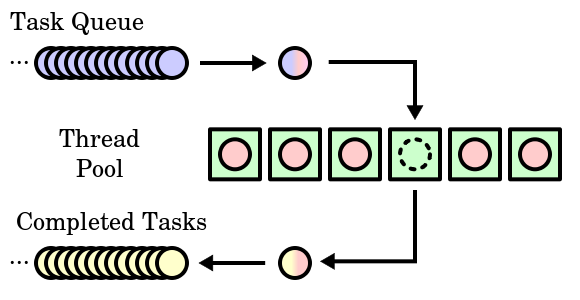
\includegraphics[scale=0.5]{images/threadpool.png}\newline
    \caption{Agencement d'un bassin de processus.}
\end{figure}

Le problème de plusieurs processus est qu'ils prennent plus de mémoire, ayant chacun leur espace mémoire là où celui-ci aurait pu être partagé. De plus. chacun des objets scanners doit être copié
au sein du processus avant que le travail ne puisse être lancé. Après un certain temps de traitement, ces copies peuvent être extrêmement lentes.

\myparagraph{Sélection des symboles et utilisation}
La suite de l'outil est composée : du scanner en lui même et d'un sélectionneur de symboles.
Le sélectionneur prend en paramètre le chemin vers un fichier binaire, et propose à l'utilisateur de choisir, parmi les symboles accessibles au sein du programme,
lesquels sont allocateurs et lesquels sont libérateurs. Il permet également de sauvegarder dans un fichier ces choix dans le même format que celui pris par le scanner.
\begin{figure}[h]
    \centering
    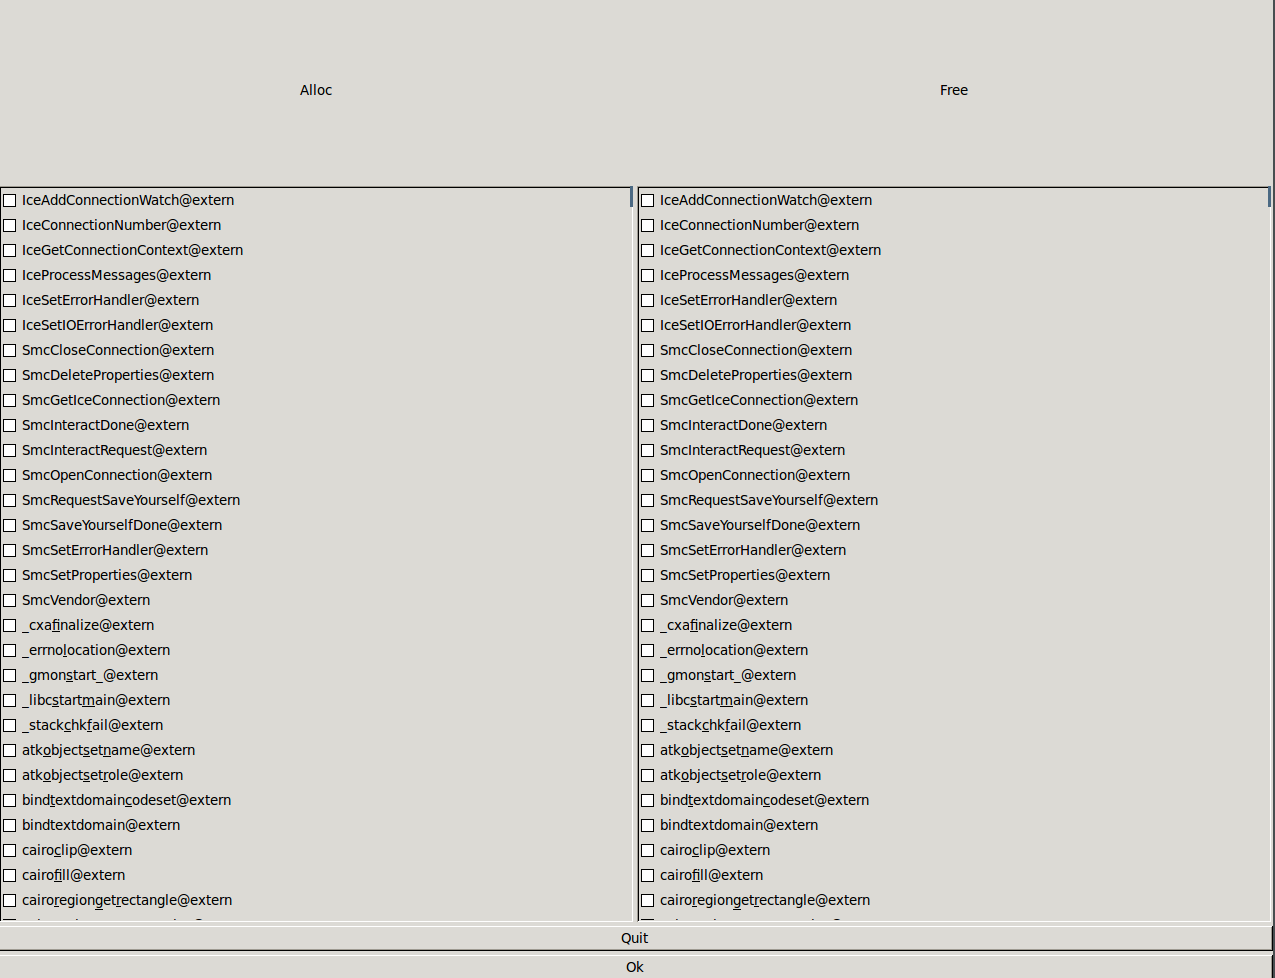
\includegraphics[scale=0.3]{images/symbol-chooser.png}\newline
    \caption{symbol-chooser.py}
\end{figure}

\subparagraph{Le Scanner}
Le fichier \textbf{parse.py} est le point d'entrée de l'outil. Il permet d'afficher le graphe relatif à un programme, de personnaliser les fonctions marquées, ainsi que de préciser
le point d'entrée de l'analyse.
\begin{figure}[h]
    \centering
    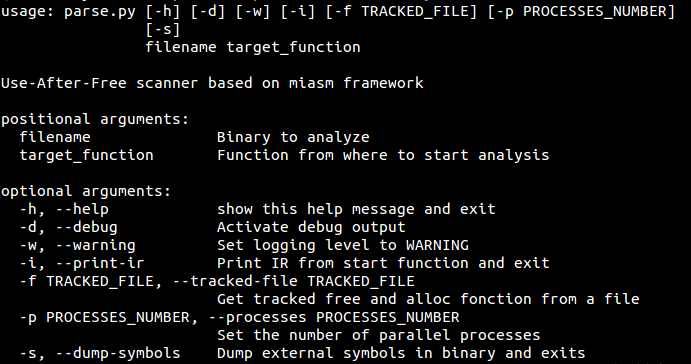
\includegraphics[scale=0.7]{images/options-parse.png}\newline
    \caption{Options de l'outil}
\end{figure}
Les journaux de déboguage sont affichés sur la sortie d'erreur du programme. Le résultat final est affiché quand à lui sous forme de rapport sur la sortie standard à la fin de l'exécution.
\begin{figure}[h]
    \centering
    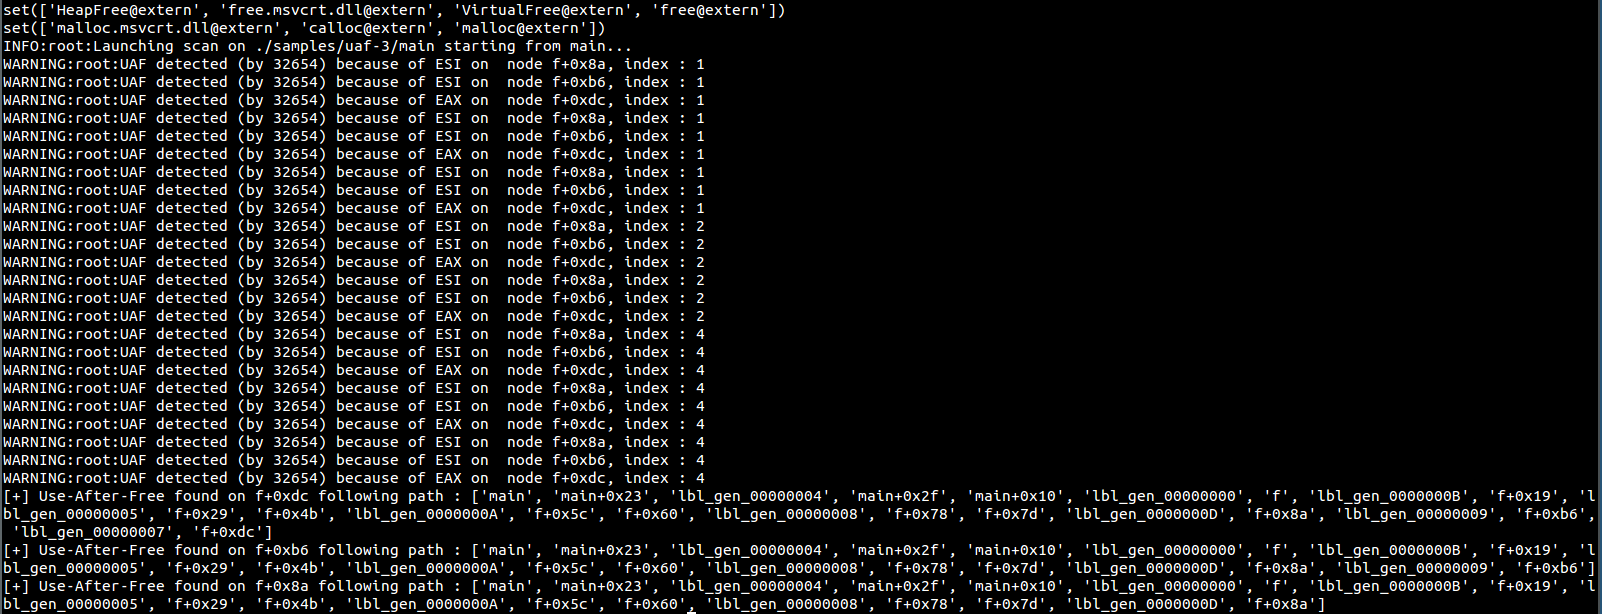
\includegraphics[scale=0.6]{images/results.png}\newline
    \caption{Exemple de résultat.}
\end{figure}
\myparagraph{Accomplissement annexes}
Miasm et Elfesteem sont deux projets sur lesquels se reposent l'outil présenté dans ce rapport. Miasm comportait quelques comportement ne satisfaisant pas à l'utilisation qui en a été faite,
il a été proposé plusieurs corrections / améliorations / changements à son auteur. Dans l'absence de réponse, un clone du projet a été créé et est disponible publiquement avec les changements.
Elfesteem quant à lui comportait un problème lors de l'analyse de binaire 64bits au format ELF. À un certain endroit, un pointeur 32bits étaient attendu par Elfesteem alors que le format
exige un pointeur 64bits. La correction a été acceptée et intégrée au code source.

\section{Interprétation et critique des résultats}
Malgré un travail qui n'est pas fini parfaitement, les fonctionnalités actuelles sont satisfaisantes et couvrent un large domaine, surtout pour les bases quasi-nulles de début de stage.
Même si la prise en main de Miasm a été laborieuse, du fait du manque de documentation et de certains non-sens selon moi, et qu'Angr semble finalement beaucoup plus approprié, aucune modification de code n'a été faite à la légère.
C'est à dire que l'ensemble des corrections sont propres et ne se basent pas sur des modifications internes importantes.
\subparagraph{}
L'analyse en sécurité demande une connaissance approfondie du language utilisé, et malgré de bonnes bases, certains comportement de Python (GIL, \_\_slots\_\_) ont demandé du temps de compréhension
et ont été parfois un obstacle au bon développement de l'outil. Le projet en lui même a requis des connaissances dans de divers domaines de l'informatique, comme par exemple la théorie des graphes.
La recherche dans tous ces domaines a demandé également un certain temps.
\subparagraph{}
Même si l'outil n'est pas raisonnablement utilisable sur de gros projets, il peut l'être sur des binaires avec une taille plus réduite (lecteur de PDF simple, etc.).
\subparagraph{}
L'ensemble est assez documenté et commenté pour permettre une reprise du travail effectué  dans le futur. Une partie du développement a également été réservée pour prendre
soin de découper le projet en fonction indépendante et modulaire, d'éviter la surcharge et de faciliter la compréhension. Une poursuite du travail pourra notamment rendre l'outil fonctionnel sur des
solutions à plus grande échelle.

\myparagraph{Point de vue personnel et apprentissage}
Ce stage m'a permis d'évoluer et de couvrir la sécurité technique sur son ensemble, et de manière assez approfondie. La première partie du stage, durant laquelle j'ai passé beaucoup de temps à
regarder le fonctionnement en détail des systèmes d'exploitations Windows / Linux et leurs allocateurs mémoires a été très formatrice. Le sujet de stage en lui même m'a permis de me diversifier sur
d'autres problématiques que la sécurité en elle-même, avec de la théorie des graphes, des problèmes d'optimisations mémoire, etc.
\subparagraph{}
L'équipe en charge des tests d'intrusion ou celle de la R\&D ont toujours été disponibles pour répondre à mes questions, et les différentes présentations organisées par les membres (NTFS, Python sur Windows, Wow64, etc.)
permettent de monter en compétence sur d'autres domaines que le sujet de stage n'aborde pas ou peu.
